\section{Event Data Handling and Data Processing}
\label{sec:datahandling}

%Ideally, we should split this chapter in two. 
% - Data handling should contain a descriptions of the data handling tools (metacat, Rucio, DeclaD,...) and the production system
% - A Data processing chapter should discuss the workflow described here

%\red{Add about cache (see g-2 cache) to improve pre-staging speed}
%\red{Say something about contingency plans to recover lag in processing}

This section covers the workflow to process the data produced by the DAQ system, the tools to handle the data files, and the production system to automate these operations. The files written on the DAQ buffer disk are automatically transferred to offline storage, and the first reconstruction pass (\passone) is run with the same conditions used by the trigger algorithms. Once completed, the calibrations constants are re-evaluated and updated in the condition database. The main physics streams are then reprocessed using the latest conditions, and reduced datasets are finally produced for further analysis. These different steps proceed in parallel: newer data are processed through the first reconstruction pass while older data are simultaneously reconstructed with the second reconstruction pass to maximize the data throughput. An overview of the data processing workflow is shown in Fig.~\ref{fig:workflow}. 

\begin{figure}[ht!]
  \centering
  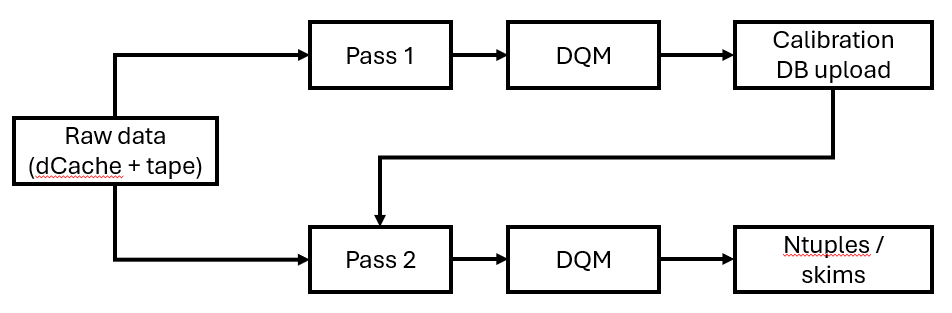
\includegraphics[width=0.95\textwidth]{figures/WorkflowOverview.png}
  \caption{Schematic of the Mu2e data processing workflow}
  \label{fig:workflow}
\end{figure}

\subsection{Data Logging and production system}
%Data logging will be supported by a set of services to catalog file properties, transfer files between storage locations, and manage production tasks: Metacat, Rucio, and DeclaD. 
The data logging system brings data from the DAQ disks to the archival storage facility and distributes it to the various computing elements. The components include a file transfer agent to transfer data from the DAQ system, a replica manager orchestrating transfers between storage elements, a metadata catalog keeping track of the data types, and interfaces to deliver the appropriate files to workflow management systems and interactive users. The existing Mu2e data catalog, sequential access via metadata (SAM), was designed for the previous generation of collider experiment at FNAL, then adopted by many intensity frontier experiments. This system is currently replaced by a new system based on Rucio, Metacat, and DeclaD.

MetaCat~\cite{Mandrichenko:2021spd} is a general-purpose metadata catalog storing permanent file description information, with location and delivery handled by Rucio. Metacat provides four major functions: store metadata associated with a file; provide a mechanism to retrieve these metadata; efficiently query the metadata database to find fill matching a list of predicates; and provide a mechanism to integrate metadata stored into external sources to query the database. The last functionality allows, for example, to seamlessly find a set of files matching criteria stored in a condition or run database. The metadata representation is flexible enough to accommodate a wide range of types and complex structures, and the catalog can scale to several hundred million entries.

Rucio~\cite{Barisits:2019fyl} is a replica manager system designed to centrally manage large volumes of data backed by many heterogeneous storage backends. This system was originally developed by the ATLAS experiment and has now been deployed to several other HEP and astronomy experiments. In a distributed system where data are physically stored over a multitude of storage servers, potentially each relying on different storage technologies (SSD/Disk/Tape/Object storage), Rucio provides an interface enabling users to interact with the storage backends in a unified way. The data can be accessed interactively or in batch jobs, and the closest file replica to the running job is delivered via streaming. Rucio is a rule-based system, allowing users to define high-level rules such as "keep 3 copies on 2 different continents". If one copy is lost, the system will automatically reconstruct the data on a different storage to maintain the rule. 

DeclaD, the Declaration Daemon, is a file transfer agent used to drain files from a set of directories and store the corresponding information in Rucio and Metacat. DeclaD is used to transfer files from the Mu2e DAQ disks to dCache. The automated follow-on processing (\passone) is discussed below.

Data processing will primarily utilize two types of storage: dCache and tape. dCache is a distributed, multi-petabyte scalable disk storage system with a single rooted filesystem providing location-independent file access. The dCache storage is readable and writable from grid machines via xrootd and transfer mechanisms such as Intensity Frontier Data Handling (ifdh). It is expected to be the main storage element for the output of distributed production jobs. The dCache scratch area is used mainly for output produced from grid jobs and files are automatically removed based on a policy with a typical lifetime of one month. The dCache persistent volume is an area for persistent storage of user files (e.g. files must be removed by their owner). The dCache tape-backed volume is a disk cache sitting in front of the tape system to prestage files written to tape. The tape storage infrastructure provides long-term storage. The current tape storage software, Enstore, provides access to data over the wide area network through the dCache disk caching system. Fermilab is actively pursuing a transition to using the CERN Tape Archive (CTA) software.

The files produced by the DAQ system will be written to persistent dCache, and most of them will be immediately copied to tape-backed dCache. The copy in persistent dCache is needed to ensure that the file is on disk when \passone\ reconstruction starts. This copy will be deleted once processing is complete. Several data streams contain pedestal data from the CRV or pre-scaled raw and intermediate data from the ExtMon and MSTM. Depending on the DOE data retention policy and the need of the sub-systems, these data might only need to reside in persistent dCache for a short period of time, without being written on tape. The final strategy will be elaborated closer to data taking. Other streams might also produce small data files (e.g. off-spill triggered events or the Error/Debug Stream) and could only be rarely accessed. These files will be held in persistent dCache for some time, perhaps a few days, and concatenated before being written to tape to make efficient use of this media. We plan to concatenate the Error/Debug stream into a single art file and to make compressed tar files of the DQM output and log files. Once transferred, the persistent dCache copy will be given an expiry date.

The production system is used to streamline data processing. It automatically detects new entries in the file catalog and launches the corresponding processing tasks. A prototype of the data production system has been developed with previous generation technologies: SAM (file catalog), FTS (file transfer agent), and POMS (Production Operations Management Service) supporting multi-stage workflows. It has been in operation for about a year to record and process data from the cosmic ray veto test stands. The system is also ready to support upcoming sub-detector Vertical Slice Tests. 

The transition to the new data handling tools is in progress, and  preparations for Rucio and Metacat are nearly complete. Several possibilities are currently considered to replace POMS by a new job management system. Requirements on this system have been defined, emphasizing robustness and accessibility to ensure that data production can be easily managed by non-experts. A decision on the choice of technology is expected in the coming weeks, with the goal of producing a first prototype well in advance of the cosmic ray data taking.    


\subsection{\passone}
\passone\ is the first stage, starting almost immediately after the data have been transferred from the DAQ buffer disks to dCache. It will process the totality of triggered events through the full set of offline reconstruction algorithms using the same conditions information used by the trigger algorithms. The following outputs will be produced:
\begin{enumerate}
 \item The main physics output file, which will contain events with signal-like tracks, for both $\mu^-\to e^-$ and $\mu^-\to e^+$, plus events of interest for background studies.
 \item Calibration files with events needed for the various calibration algorithms.
 \item Offline DQM information (see Section~\ref{sec:monitoring}) with higher statistics and more complete coverage than that provided by the online DQM system.
 \ item Optionally, a file containing all data for debugging and validation purposes
\end{enumerate}
When necessary, the workflow will include stages to concatenate small output files into a single large file, e.g., off-spill events (there is a competing demand to produce prompt offline DQM information, and the optimal concatenation policy will be determined by the operational constraints).

Once a new run is started, the \passone\ workflow will start as soon as curated information from the online database is available. As the data logging system delivers files, the production system will monitor the file catalog and launch grid jobs to process new files (either a single or many files in one job). Under normal conditions, the jobs should be launched 10 minutes or less after the files have been cataloged and complete within 2 to 3 hours after submission. However, this time distribution is expected to have (long) tails during periods or peak usageor if the system requires maintenance. Offline DQM information will be summarized in both timelines and metrics, and out-of-tolerance data will generate an alarm. The histograms and TTrees from which these metrics are derived will be retained on disk for a certain time and persisted on tape. Files in the Error/Debug stream will also be copied to tape, concatenated if necessary, and retained on disk for inspection by experts for a limited amount of time. These events won't be further processed.

The normalization file stream includes the Intensity stream and the summary data from the ExtMon and the STM. These streams contain information to evaluate the proton bunch intensity variations over the course of each spill. These data are needed to assess the reconstruction efficiency accurately and properly normalize the results. These streams have sparse per-event information (i.e. not all information is available for every event). In addition, packaging small data products as objects in an {\tt art::Event} is inefficient in both disk/tape space and access time. One possibility might be to organize the data around spills, and the resulting information could be persisted in a database or included in each art SubRun object. Final decisions will be taken as the design matures. For these files, \passone\ will package the information in a way that is convenient for downstream processing, and concatenate input files if necessary.

The first class of low-level calibration streams includes the prescaled raw and intermediate data from the monitors and the calorimeter pulser events. The corresponding \passone\ workflow will be defined by the detector teams, but the output should include DQM and updated condition information that will be uploaded to the condition database. The input files might only be stored in dCache for a limited amount of time. The second class of low-level calibration streams contains STM waveform data for pulses with energies near the important lines. The STM team plans to periodically refit these pulses with updated conditions information to improve the estimate of the stopped muon yield. This data will be written to tape, with file concatenation when necessary.


\subsection{Calibration}
The data workflow continues with the calibration step, using the data directly produced in \passone to update the detector calibration constants. A detailed description of calibration procedures is given in Section~\ref{sec:calibration}. Most of the time, the output of \passone\ should be sufficient to perform this work. However, it may be necessary to re-run a subset of \passone\ using the conditions information determined by the previous pass, and repeat the procedure until the calibration information has converged. This might be required, for example, during commissioning and early data taking. When necessary, the subsystem will be able to run repeated \passone\ jobs using the data production system. Once calibration are certified, the offline condition database is updated. The online condition database is periodically synchronized to the offline database.


\subsection{\passtwo}
Once calibrations for a time interval are certified, the main physics streams (on-spill and off-spill triggered events) are reprocessed using updated conditions information. This operation is called \passtwo and will produce a new set of DQM information and output data files. During commissioning and early data taking, \passtwo might perform the full reconstruction from the raw data. As we gain experience, it might become possible to only refit existing tracks and recalculate the parameters of existing calorimeter clusters and CRV stubs. In that case, the raw data in the output of \passone\ could be filtered to only include the necessary information.

Based on experience with previous experiments, Mu2e expects the following three-week cycle as the start of the experiment: take data for week N, run calibration jobs for data taken during week N-1, and run Pass2 for week N-2 data. As data taking becomes stable, it may be possible to compress this time scale. During a year-long run, we also expect continuous improvements in calibrations and reconstruction algorithms. When integrated improvements warrant it, we will re-run \passtwo\ on all recorded data.


\subsection{Reduced data sets}
The data workflow ends with the production of reduced data sets. The format and use cases are discussed in Section~\ref{sec:analysis}. There may be several types of datasets, each targeted to a particular analysis task. These data sets will be directly produced from the output of \passtwo, running additional reconstruction algorithms if needed. They will be produced for every iteration of \passtwo. As analysis algorithms evolve, reduced data sets will be reproduced to reflect these improvements. The output of \passtwo and reduced data sets should be small enough that this step will not require significant resources.

Additionally, skim data sets may also be produced from the output of \passtwo. Each skim data set contain a fraction of the original data, selected by a dedicated filter and preserving the full information of the original event. These data sets would reduce computing needs and processing times during the analysis phase.   
